\clearpage
\VerdierPhysicalPageAnchor{0083}%
\VerdierSemanticAnchor{ch1-3-1-1-additivity}
圏 $\operatorname{tr}_1(C)$ は加法圏である。$X\xrightarrow{f}Y$ と
$X'\xrightarrow{f'}Y'$ の直和は

\VerdierSemanticAnchor{ch1-3-1-1-direct-sum}
\begin{equation*}
  X\oplus X'
  \xrightarrow{\left(\begin{smallmatrix}f&0\\0&f'\end{smallmatrix}\right)}
  Y\oplus Y'
\end{equation*}
である。

\VerdierSemanticAnchor{ch1-3-1-2}
\noindent\textbf{3.1.2.}\quad
$X\xrightarrow{f}Y$ を $\operatorname{tr}_1(C)$ の対象とする。次のようにおく：

\VerdierSemanticAnchor{ch1-3-1-2-cone-object}
\begin{equation*}
  c(f)^i=Y^i\oplus X^{i+1},
\end{equation*}

\VerdierSemanticAnchor{ch1-3-1-2-eq1}
\begin{equation}
  d_{c(f)}^i=
  \begin{pmatrix}
    d_Y^i & f^{i+1}\\
    0 & -d_X^{i+1}
  \end{pmatrix}
  \colon Y^i\oplus X^{i+1}\longrightarrow Y^{i+1}\oplus X^{i+2}.
  \tag{3.1.2.1}
\end{equation}

\VerdierSemanticAnchor{ch1-3-1-2-cone-verification}
これにより $C$ の対象からなる複体が定義されたことが確かめられる。
\VerdierSemanticAnchor{ch1-3-1-2-cone-name}
この複体を $c(f)$ と書き、射 $f$ の\emph{写像錐}と呼ぶ。次に

\VerdierSemanticAnchor{ch1-3-1-2-morphism-setup}
\begin{equation*}
  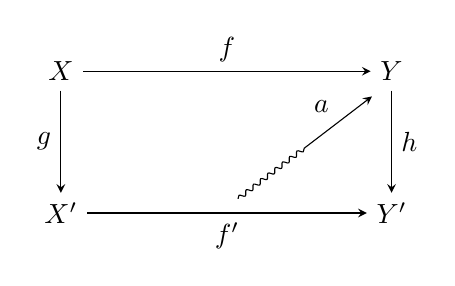
\begin{tikzpicture}[>=stealth,baseline=(current bounding box.center)]
    \node (X)  at (0,1.8) {$X$};
    \node (Y)  at (4.2,1.8) {$Y$};
    \node (Xp) at (0,0) {$X'$};
    \node (Yp) at (4.2,0) {$Y'$};
    \draw[->] (X) -- node[above] {$f$} (Y);
    \draw[->] (X) -- node[left] {$g$} (Xp);
    \draw[->] (Y) -- node[right] {$h$} (Yp);
    \draw[->] (Xp) -- node[below] {$f'$} (Yp);
    \draw[decorate,decoration={snake,amplitude=0.8pt,segment length=3.3pt}]
      (2.25,0.18) -- (3.10,0.83);
    \draw[->] (3.10,0.83) -- node[above left] {$a$} (3.95,1.48);
  \end{tikzpicture}
\end{equation*}
を $\operatorname{tr}_1(C)$ の射とする。次のようにおく：

\VerdierSemanticAnchor{ch1-3-1-2-eq2}
\begin{equation}
  c((g,h,a))^i=
  \begin{pmatrix}
    h^i & a^i\\
    0 & g^{i+1}
  \end{pmatrix}
  \colon Y^i\oplus X^{i+1}\longrightarrow Y'^i\oplus X'^{i+1}.
  \tag{3.1.2.2}
\end{equation}

\VerdierSemanticAnchor{ch1-3-1-2-complex-morphism}
これらの射は $c(f)$ と $c(f')$ の微分と可換であり、したがって複体の射

\VerdierSemanticAnchor{ch1-3-1-2-eq3}
\begin{equation}
  c((g,h,a))\colon c(f)\longrightarrow c(f')
  \tag{3.1.2.3}
\end{equation}
を定める。

\VerdierSemanticAnchor{ch1-3-1-2-cone-functor}
このようにして関手
$c\colon\operatorname{tr}_1(C)\longrightarrow\operatorname{comp}(C)$
が定義されたことが確かめられる。これを\emph{写像錐関手}と呼ぶ。

\VerdierSemanticAnchor{ch1-3-1-2-s-functor}
$s\colon\operatorname{comp}(C)\longrightarrow\operatorname{tr}_1(C)$ を
関手 $X\longmapsto(0\longrightarrow X)$ とする。
\VerdierSemanticAnchor{ch1-3-1-2-phi-setup}
$\operatorname{tr}_1(C)$ の各対象 $X\xrightarrow{f}Y$ に対し、
$\Phi(f)\colon(X\xrightarrow{f}Y)\longrightarrow s c(f)$ により
